\chapter{Moving to the Web}
\label{chap2}

We decided to build the Giflang's interpreter and the IDE for web and we tried to move as much code to the client side as possible. This chapter explains
why we decided to do so.

A growing number of applications are being implemented for web browsers (as opposed to using native OS interfaces). Google is even building an
operating system called ChromeOS based around their market-dominating browser Chrome. With modern Web APIs, apps that were previously
thought of as typical native OS apps are now moving to the browser. Below are a few examples of such apps:
\begin{enumerate}
\item Photopea \cite{Photopea} -- A Photoshop web alternative
\item Google Hangouts \cite{Hangouts} -- A pioneer WebRTC\footnote{WebRTC (Web Real-Time Communication) provides web browser 
applications with real-time communication (RTC) via simple APIs.} app providing realtime video communication
\item TODO: Add an in-browser FPS here
\end{enumerate}

\section{Native vs Web IDE}
Most well known IDEs (e.g., Visual Studio, Eclipse or Xcode) are native OS (Operating System) applications. Web IDEs such as REPL.it or Ideone, on the other hand,
are not very widespread. We think that this is because users usually want to edit local files while browsers have limited support for reading
and saving local files programmatically. There is no Web API to overwrite a file at a given location on a user's disk for example.
Browsers prohibit this to protect the user's security.

Giflang is not suited for use in any serious project development and it is also not intended for such use. It is meant for creating a
challenging and fun environment for solving programming problems. The standard I/O can be used for accepting problem inputs and writing results.

Therefore, Giflang does not have to support file I/O, multi-source programs and other otherwise-standard functionality. Of course later
on, a graphical output, file I/O or other features can be added, but within the scope of this thesis we only plan on supporting
the basic functionality.

Considering the above paragraphs we concluded that a web IDE is more suitable for our type of application since it offers benefits as
ease of access and an installation-free setup. In our opinion, this outweighs the advantages of native IDEs such as easy local disk
file access and ability higher performance.

\section{Client side vs server side interpreter}

The Giflang code can be either interpreted on the server side or client side. By server side we mean any code that runs on the server. This means that
the interpret could be written in almost any language using any technologies, because it is up to us to choose what we run on the server. On the other hand,
client side code is executed in the browser which can only run JavaScript or WebAssembly.

\subsection{Server side execution}
Executing code on the server side means that in order to interact with it, for example provide an interactive input or see a gradual output, the browser and
the server need to communicate during the execution. There are $2$ basic approaches to this communication:
\begin{enumerate}
\item HTTP polling -- the client (browser) initiates the communication to the server and waits for a response
\item WebSockets -- the client and the server open a two-way channel (WebSocket) through which the server can send messages to the client without
the client sending a request 
\end{enumerate}

\begin{figure}[!hbt]
	\includegraphics[width=\textwidth]{../img/websockets}
	\caption{A visualization of HTTP polling and WebSockets}
	\label{fig:chap2:websockets}
\end{figure}

We will introduce two Web IDEs that use server side execution -- REPL.it and Ideone. They both support numerous languages such
as Python, C, C++ and Java.

Ideone uses HTTP polling to get updates about the execution. Firstly, it sends a request to the backend containing source code and input.
After that, it polls the server for an update every second. The server can respond with a new output, an error report, a finish status, etc. Users of Ideone need to
specify all the output at once before the start. While it would be possible to implement an interactive I/O with the polling, Ideone chose not to do so.
We did not find out why.

Having to poll the server for updates is awkward. If the granularity of polling is high, requests are send frequently, but
in between consecutive requests the state might not have changed. That results in wasting resources. On the other hand, if the granularity is low, less
requests are send, but that might result in higher latency between a state change happening on the server and the client picking it up.

WebSockets address this issue. They allow opening a two-way interactive communication session between the user's browser and the server.
Using this API, the browser can send messages to the server and receive event-driven responses without having to poll the server for a state\footnote{source: mdn todo}.
We can see this in Figure \ref{fig:chap2:websockets} where the WebSocket communication is marked with red arrows.
Before WebSockets were introduced around the year 2012, there was no way to initiate a communication from the server to the browser as HTTP is a request-response
protocol. This means that servers could only respond to browser's requests.

REPL.it is more modern compared to Ideone and uses WebSockets. It also provides an interactive I/O and debugging.

\subsection{Client side execution}
By default, the browser uses a single thread -- also called the main thread -- to run all the JavaScript of a webpage, as well as to perform layout
changes, reflows, and garbage collection. As a result of this, long-running JavaScript functions can block the thread, leading to an unresponsive
page.\footnote{source: mdn}

\subsubsection{WebWorkers}
Running the interpreter in the main thread would take processing time from UI updates which could lead to a bad responsiveness of the page. To
address this issue, browsers adopted support for WebWorkers. WebWorkers allow us to run scripts in the background threads, leaving main thread
to handle UI-related tasks.

Sharing data between threads is typically achieved by accessing the same piece of memory. However, the communication between WebWorkers and the main
thread is achieved via messages:
\begin{code}
// Main script
var myWorker = new Worker('worker.js');
myWorker.postMessage('Hello Worker');

// worker.js
onmessage = function(msg) {
  console.log('Got a message from main: ' + msg);
}
\end{code}

An interpreter running in a separate WebWorker does not take processing time from the UI tasks in the main thread. We could not find an existing
project that would interpret or compile code in a WebWorker.

\subsubsection{WebAssembly}
JavaScript in the browser is executed by a JavaScript engine. Different browsers might have different engines. As Figure \ref{fig:chap2:v8_bench} shows,
JavaScript engines like V8 or SpiderMonkey keep improving in terms of speed. Nonetheless, a program written in a language
with highly optimized compiler like C++ or Rust that compiles to the machine code will most probably outperform any JavaScript engine.

\begin{figure}[!hbt]
	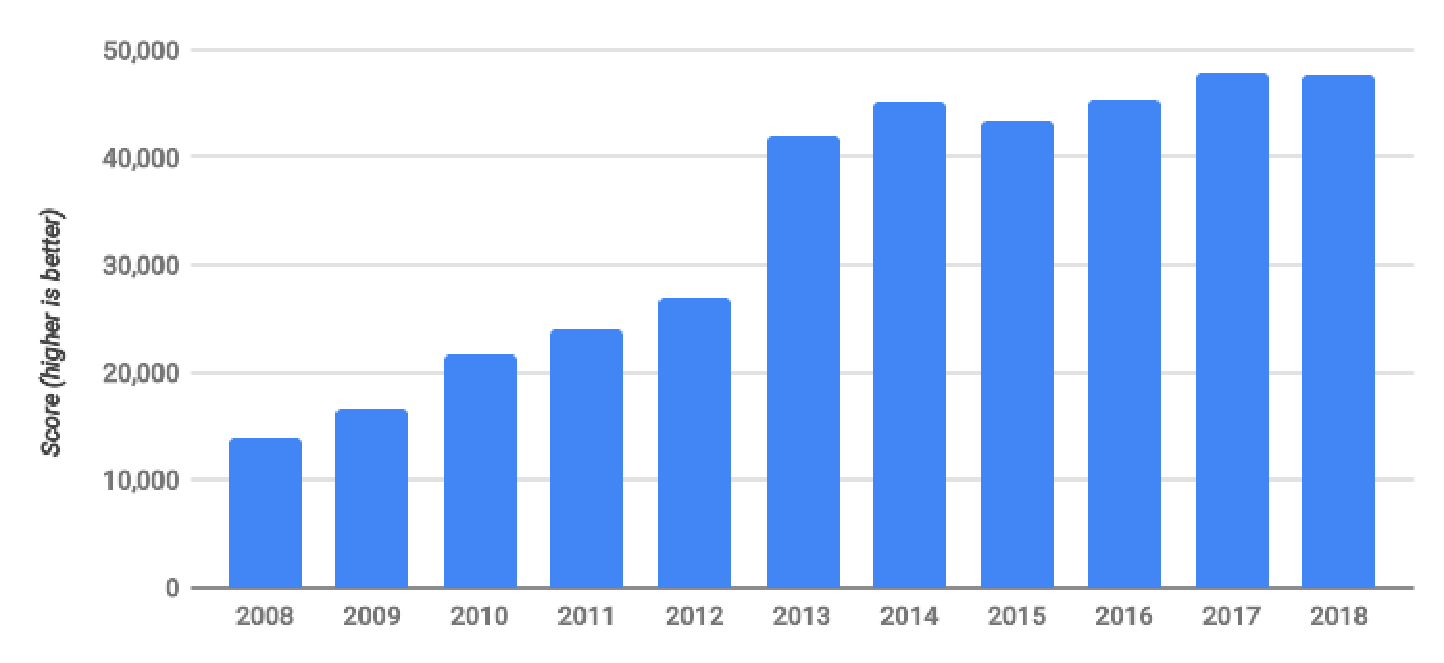
\includegraphics[width=\textwidth]{../img/v8-bench}
	\caption{A chart showing V8 improving over the years. Source: \href{https://v8.dev/blog/10-years}{v8.dev}}
	\label{fig:chap2:v8_bench}
\end{figure}

In order to close the gap between computational-heavy programs executing well natively while poorly in browser, WebAssembly
language was introduced in 2015. WebAssembly is a low level language that is now supported by all major browsers. Since it is
close to the machine code, it is meant to be a compilation target language of other higher level languages.

Currently, many languages such as C/C++, Rust or TypeScript, can be compiled to WebAssembly. These compilers usually also emit
a \emph{glue code} that contains handles that allow calling functions defined in the WebAssembly code from JavaScript.

Integrating functions defined in WebAssembly into a JavaScript script requires non-trivial effort since only primitive types can be passed
as function arguments and return values.

There are many ports of existing interpreters and compilers to WebAssembly, because there are tools like Emscripten\footnote{Add reference}
that can compile C/C++ code to WebAssembly; for example we really like Iodide\footnote{Todo reference} -- a project that brings scientific Python
to the client side of the browser.

\subsection{Conclusion}
The advantage of server side interpreter is speed as the interpreter can use almost any technology. Web IDEs typically choose
server side execution for different reason, though. It is simpler than implementing interpreters for given languages in JavaScript or
porting the existing interpreters to WebAssembly. Since in our project we do not care so much about execution speed and
we do not have an existing interpreter or compiler, we can do better than server side execution.

The client side execution requires no special support from the server and it also works offline, i.e., after user looses connection. Running an interpreter
compiled to WebAssembly in a WebWorker would be the best approach as it would provide performance and also offloading from the main thread.
However, when we started working on the thesis we did not have any prior experience with writing an interpreter and adding another layer into the stack in the
form of WebAssembly seemed very complex. It would allow us to use a language like C++ or Rust for the development. To keep things simpler we
decided to write the interpreter in JavaScript and run it in a WebWorker.

\section{Picking the right Javascript flavour}
JavaScript started evolving again in 2015, when a new standard -- ECMAScript 2015 -- was published. Prior to that, the last prominent
standard was introduced in 2009. Currently, there is a new standard released every year. With all the new additions to the language, programming in
JavaScript nowadays is way more pleasant than ever before.

However, it is still a dynamically typed language. Since we prefer statically typed languages we looked into the options of writing client-side scripts in
a statically typed language. It seems like every Silicon Valley tech giant tried to bring types to JavaSript. Google created Dart,
Facebook made Flow and finally, Microsoft created TypeScript. All of these languages can be transpiled to JavaScript while enforcing the static types.

Dart is a Java-like programming language, quite far from JavaScript in terms of its syntax. Flow lets programmers
annotate a JavaScript code with types and enforce them. TypeScript is similar to Flow, but it is more popular and has a bigger community.

From the languages described above we picked TypeScript, mainly because as of now it has a lot of momentum and it is being widely adopted.

\section{The rise of single-page applications}
In the old days of the web, before the year 2000, any data exchange between a server and a browser required reloading an entire page. 
Ajax\footnote{Asynchronous JavaScript + XML} was introduced to solve this problem by allowing web applications to send and retrieve data from
a server asynchronously (in the background), without interfering with the display and behavior of the existing page\footnote{wikipedia}.

Ajax later gave rise to single-page applications (SPAs). SPA is a web application that interacts with the user by dynamically rewriting
the current page rather than loading entire new pages from a server\footnote{wikipedia}. In this thesis, we build an SPA, because users should not
face any page-reloads while interacting with a web IDE (e.g., when running or saving the code).  

Browsers were originally designed for a stateless page-redraw model and thus with SPAs some new challenges emerged. The most predominant of them is
probably keeping the displayed UI in sync with the app's state.

Let us show what we mean by keeping the state in sync with the UI on a simple example. Consider a widget for creating a list of emails like one shown below.
Users can add emails and delete them later. This example is inspired by the one shown in the article \cite{JSFramework}.
\begin{figure}[!hbt]
    \centering
	\includegraphics[width=0.5\textwidth]{../img/emails}
	\caption{A simple widget for creating a list of emails}
	\label{fig:chap2:emails}
\end{figure}

We can represent the state of this application as a list of emails with a unique ID. Below is a JavaScript object holding the state displayed in
Figure \ref{fig:chap2:emails}.
\begin{code}
let state = [
    { email: 'john@doe.com', id: 0 },
    { email: 'petr@novak.cz', id: 1 },
    { email: 'sample@email.sk', id: 2 },
]
\end{code}

Every user action that changes the state has to also update the UI accordingly. Adding an email should add it to the state object, but also update
the DOM\footnote{The Document Object Model (DOM) is a programming interface for HTML and XML documents.} by appending a new element to the email list.
Similarly, removing an email should remove it from the list and from the UI.
\begin{code}
// DOM nodes of the list.
let li_items = []
// List of emails with IDs.
let state = []

function addEmail(email) {
    // State change
    const id = GetNextId()
    state = state.concat({ email, id })

    // UI change
    const ul = document.createElement('ul')
    const li = document.createElement('li')
    const span = document.createElement('span')
    const del = document.createElement('a')
    span.innerText = email
    del.innerText = 'delete'
    del.setAttribute('data-delete-id', id)

    ul.appendChild(li)
    li.appendChild(del)
    li.appendChild(span)
    li_items[id] = li
}

function removeEmail(id) {
    // State change
    state = state.filter(item => item.id !== id)

    // UI change
    const ul = document.createElement('ul')
    ul.removeChild(li_items[id])
}
\end{code}

This example is very basic, but for more complex apps with bigger states, it is very easy to end up with the UI and the state out of sync. It is the case
because we have to write code for both the state change and the UI change. JavaScript frameworks abstract away the fact that UI needs
to be updated accordingly when the state changes. They simply give a guarantee that whenever the state is mutated, the UI gets updated.

\subsection{React}
React \cite{React} is a JavaScript framework created by Facebook. To make sure the UI corresponds to the state, the whole UI is re-rendered
when the state changes. However, re-renders are costly operations and deleting the whole DOM and creating a new one from scratch on every re-render
would be very slow. Instead, React renders the page into a Virtual DOM. Virtual DOM is a “virtual” representation of a UI kept in memory and
synced with the “real” DOM by React\footnote{React docs}. This process is called reconciliation.

The reconciliation takes the current Virtual DOM and a snapshot of the last synced Virtual DOM and tries to find the minimum number of operations to turn
one into another. There are some generic solutions to this algorithmic problem of generating the minimum number of operations to transform one tree into another.
However, the state-of-the-art algorithms \cite{TreeEditDistance} have a complexity in the order of $\mathcal{O}(n^3)$ where $n$ is the number of elements in
the tree\footnote{taken from React docs}. Therefore, React team decided to implement a heuristic $\mathcal{O}(n)$ algorithm.

\begin{figure}[!hbt]
    \centering
	\includegraphics[width=\textwidth]{../img/virtual_dom}
	\caption{A flowchart of React updating the DOM.}
	\label{fig:chap2:virtual_dom}
\end{figure}

There are many other frameworks (e.g., Angular, Vue.js, Ember.js). Each of them has a different approach to solving the UI and the state syncing. However, we picked
React for this project, mainly because we used it in previous projects where it proved itself very useful and easy to use.

\section{Storing programs}
We want to allow users to save, load and share their programs. A typical solution to this problem is to create a database in the backend. However, since all
of our application logic lies on the client side we looked into a way of opting out of creating a database and using a ready-made service. This would mean that
our backend could consist of only a server serving static files.

\subsection{Backend as a service}
Backend as a service (BaaS) is a model for providing app developers with a way to link their applications to a backend cloud storage and APIs exposed by back end
applications while also providing features such as user management or push notification.\footnote{wikipedia} These services are provided via the use of custom
SDKs\footnote{Software development kit} and APIs.

There are many different BaaS providers (e.g., Back4App, Parse Server or AWS Aurora), but we chose to use Firebase /TODO cite/ from Google. Since we do not
need a complex functionality for our project, picking almost any other provider would still work well with our app.

The biggest advantage of BaaS over a custom backend is that BaaS saves developers a lot of time as it offers user management and data storage.
Providers usually promise seamless scaling of the app. On the other hand, BaaS gives developers less control as they have to adhere to the limits of the APIs
and it can also cost more than a VPS with a custom server.

\subsection{Sharing and forking the programs}
\label{chap2:program_id}

In order to allow users sharing their programs with other users, we need to give each program a unique ID which can then be used to load the program later.
This ID can be put in the URL, for example as a GET parameter or part of the path.

When a user program is saved for the first time, it is given a unique ID. Any subsequent saves overwrite the current version. If we keep overwriting
a saved program even after a page reload, user A might load a program of user B and overwrite the work of user B.

In order to prevent users from overwriting each others' programs, we decided to always assign a new ID to a program that is saved for the first time after
a page load. This allows users to fork an existing program without having an ability to change it.

\begin{figure}[!hbt]
    \centering
    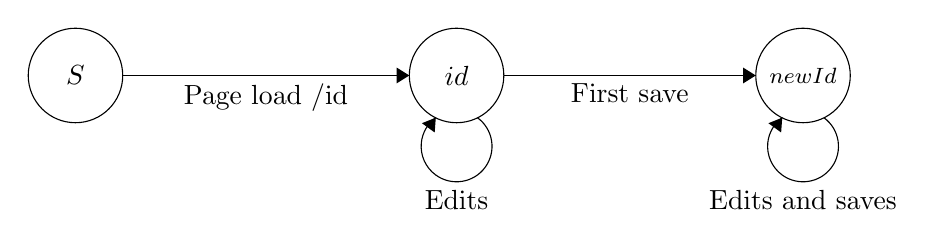
\begin{tikzpicture}[scale=0.2]
    \tikzstyle{every node}+=[inner sep=0pt]
    \draw [black] (21.4,-32.1) circle (3);
    \draw (21.4,-32.1) node {$S$};
    \draw [black] (45.6,-32.1) circle (3);
    \draw (45.6,-32.1) node {$id$};
    \draw [black] (67.6,-32.1) circle (3);
    \draw (67.6,-32.1) node {\footnotesize $newId$};
    \draw [black] (24.4,-32.1) -- (42.6,-32.1);
    \fill [black] (42.6,-32.1) -- (41.8,-31.6) -- (41.8,-32.6);
    \draw (33.5,-32.6) node [below] {Page\mbox{ }load\mbox{ }/id};
    \draw [black] (46.923,-34.78) arc (54:-234:2.25);
    \draw (45.6,-39.35) node [below] {Edits};
    \fill [black] (44.28,-34.78) -- (43.4,-35.13) -- (44.21,-35.72);
    \draw [black] (48.6,-32.1) -- (64.6,-32.1);
    \fill [black] (64.6,-32.1) -- (63.8,-31.6) -- (63.8,-32.6);
    \draw (56.6,-32.6) node [below] {First\mbox{ }save};
    \draw [black] (68.923,-34.78) arc (54:-234:2.25);
    \draw (67.6,-39.35) node [below] {Edits\mbox{ }and\mbox{ }saves};
    \fill [black] (66.28,-34.78) -- (65.4,-35.13) -- (66.21,-35.72);
    \end{tikzpicture}
	\caption{A state machine showing how program ID changes in the web IDE}
	\label{fig:chap2:page_url}
\end{figure}

JSFiddle mentioned in the Section \ref{chap1:related_work} uses the same approach. Additionally, JSFiddle also stores all intermediate versions. However,
we did not find it crucial and chose to overwrite the current version after each save, except for the initial save.
